\section{Discussion}\label{sec:phase_est_discussion}

We proposed a new approach for the control of powered transfemoral prostheses.
The approach uses a robust estimate of the gait phase derived from an EKF that
integrates multiple sensor measurements to determine the desired knee and ankle
angles, velocities and torques from trained control surfaces. The proposed
approach improved knee kinematics over NM and IMP control, matched NM control
and improves upon IMP control in terms of gait robustness to ground height
disturbances, and adapted the phase estimate to both gradual and abrupt changes
in speed more quickly than a time-based phase estimate.

We believe the robustness improvements of the proposed GP-EKF control scheme and
the NM control over IMP control stem from the smoothness of the phase estimation
in these two controllers. In NM control, the phase estimation is implicit and
encoded in the internal states of virtual muscles, which are modulated by
musculoskeletal dynamics and reflexes. In the proposed control presented here,
the EKF directly infers a robust estimate of phase from multiple measurements.
In either case, the resulting control commands are smooth and do not normally
change abruptly from one moment to the next. In contrast, IMP control splits the
stance phase into three discrete phases that are triggered by joint angle
thresholds.  Consequently, in the ground height disturbance experiments,
subjects were occasionally caught off-guard by unexpected transitions, triggered
by abnormal kinematics when stepping on a block, which then caused large, sudden
changes in torque. Unexpected phase transitions between the mid-stance and
late-stance phases were especially consequential, as in the late-stance phase,
knee torque trends towards zero to allow for passive knee flexion, while the
ankle plantarflexes. If a user's center of mass is positioned incorrectly, this
combination of joint torques can cause a sudden collapse of the knee, which was
the cause for many of the observed falls with IMP control. 

NM control too can result in unexpected falls due to incorrect phase estimation.
The experienced user fell a total of eight times when stepping on blocks with
the NM control (see square marker~\cref{fig:num_block_falls}). These falls were
the result of a modelled reflex that reduces knee extensor muscle stimulation in
late stance in proportion to ankle plantarflexion, thereby allowing for passive
knee flexion leading into swing. In contrast to less experienced subjects, the
experienced user was able to control the knee over-extension during stance and
achieve more normal knee flexion in late-stance during normal walking
(see~\cref{fig:controller_comparison} row 1, column 2), However, this increased
knee flexion during normal walking may have increased the prosthesis'
susceptibility to premature knee collapse when disturbed. While the modeled
neuromuscular reflexes seem to work well during steady-state walking and during
disturbed walking for inexperienced users, the large increase in falls for the
experienced user, exposes the difficulty of relying on heuristic reflexes to
obtain robust control across a range of gait characteristics. In contrast, the
proposed EKF approach takes a principled approach to phase estimation and thus
resulted in the fewest falls.

\begin{marginfigure}
    \centering
    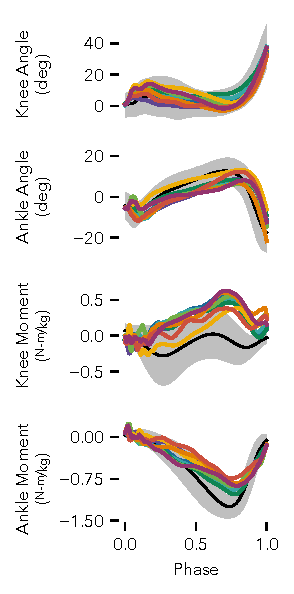
\includegraphics[width=\linewidth]{normal_data_fixed_ankle}
    \caption{GP-EKF phase control with fixed control surfaces and
    increased ankle impedance.}\label{fig:gp_ekf_fixed}
\end{marginfigure}
Some improvements can be made in the implementation of the proposed control.
The normal walking experiments show that the ankle trajectories produced by the
GP-EKF control are less natural than those produced by NM or IMP control
(see~\cref{fig:kinematic_errors}b). The GP-EKF ankle trajectories
in~\cref{fig:controller_comparison} show that peak ankle flexion is achieved
later in stance and that the ankle insufficiently plantarflexes at toeoff.
There were two reasons for these issues. First, in hindsight the cutoff between
stance and swing in the data used to train the control surfaces was set too
early in the gait cycle. Second, the ankle impedance, especially in the push off
phase was too low. \Cref{fig:gp_ekf_fixed} shows the trajectories for all 9
control surfaces with corrected control surfaces and with and ankle stiffness
($k_p$ \cref{eq:pdandff}) that is roughly double of that used for the previous
results. These changes substantially improve the ankle kinematics in the push
off phase.

However, increasing the ankle stiffness throughout stance may make an overly
ridged controller that does not comply to rough terrain. Recent research has
investigated how impedance varies continuously throughout
gait~\citep{lee2016summary}. These results could be used to parameterize
impedance as a function of phase. Taking this step could help improve the
naturalness of the knee and ankle torques produced by the GP-EKF controller,
which currently trail those produced by the NM and IMP controllers
(see~figs.~\labelcref{fig:kinematic_errors}c and d).

There are several other avenues for future research to expand the proposed
control approach. First, we only used prosthesis joint angles and velocities for
the observation models. It is worth investigating if additional measurements
such as ground reaction forces, accelerations, and EMG signals improve the state
estimate.  Second, we used a simple, two-state model to represent the entirety
of the coupled human-prosthesis state during stance. Adding additional state
variables may help capture important behaviors such as balance recovery actions
taken by the upper body. To this end, dimensionality reduction techniques could
help identify better state representations from gait data. New state
representations need to satisfy two constraints that our current model
satisfies: (1) The evolution of the state needs to approximately abide by some
Markov dynamics model so we can perform the predict step of the EKF
(\cref{eq:ekf_predict_mean,eq:ekf_predict_cov}). (2) The evolution of state
throughout stance should be knowable in hindsight after a step is completed so
that the observation model can be learned online. Finally, with more advanced
state and observation models, more advanced forms of state estimation may be
necessary, including unscented Kalman filters or particle filters such as the
one proposed by \citet{dhir2018locomotion}, which allows for continuous gait
phase estimation using discrete heel and toe contact sensors. 
